\section{Introduction}
The emergence of large language model (LLM) agents marks a new paradigm~\citep{cheng2024exploring,tao2024survey,gao2025survey,fang2025comprehensive}, delivering significant improvements over static models in complex, dynamic task environments. 
Memory serves as a crucial component in prompting agent test-time self-evolution~\citep{zhang2025survey}, which provides a substrate for accumulating, organizing, and reusing past knowledge without retraining the base model~\citep{xu2025mem,tang2025agentkb}. 
% Consequently, how to design an effective memory system for agents has garnered increasing attention. 
Among memory paradigms, procedural memory is particularly attractive for agents, as it gathers high-quality problem-solving experiences from historical interaction trajectories~\citep{wang2025mirix,fang2025memp}. 
These experiences can be leveraged to guide agent decision-making in new tasks, thereby reducing redundant trial-and-error and avoiding local optima~\citep{chen2025swe} (as shown in Figure~\ref{fig:example}). 

Existing memory systems predominantly store complete trajectories as experiences~\citep{zheng2023synapse,hu2024hiagent} or summarize structured workflows~\citep{tang2025agentkb,chen2025swe,liu-etal-2025-contextual} corresponding to entire trajectories. 
However, these approaches often overlook the importance of choosing an appropriate level of granularity, since coarse-grained trajectory-level experiences may contain irrelevant information that can mislead agents into making erroneous decisions in new tasks. 
This motivates us to explore the potential of fine-grained keypoint-level experiences, which distill critical steps that influence task outcomes. 
Moreover, as task distribution shifts and agent self-improves over time, stored experiences may become inapplicable or inefficient~\citep{xiong2025memory}. 
Consequently, an effective experience refinement mechanism is essential to maintain memory quality for long-term agent performance. 
While prior works have investigated memory management strategies for LLM agents~\citep{chhikara2025mem0,yan2025memory}, they mainly require prompting or fine-tuning LLMs to select memory operations, failing to establish LLM-independent, quantitative criteria for experience addition and deletion.

\begin{figure*}
    \centering
    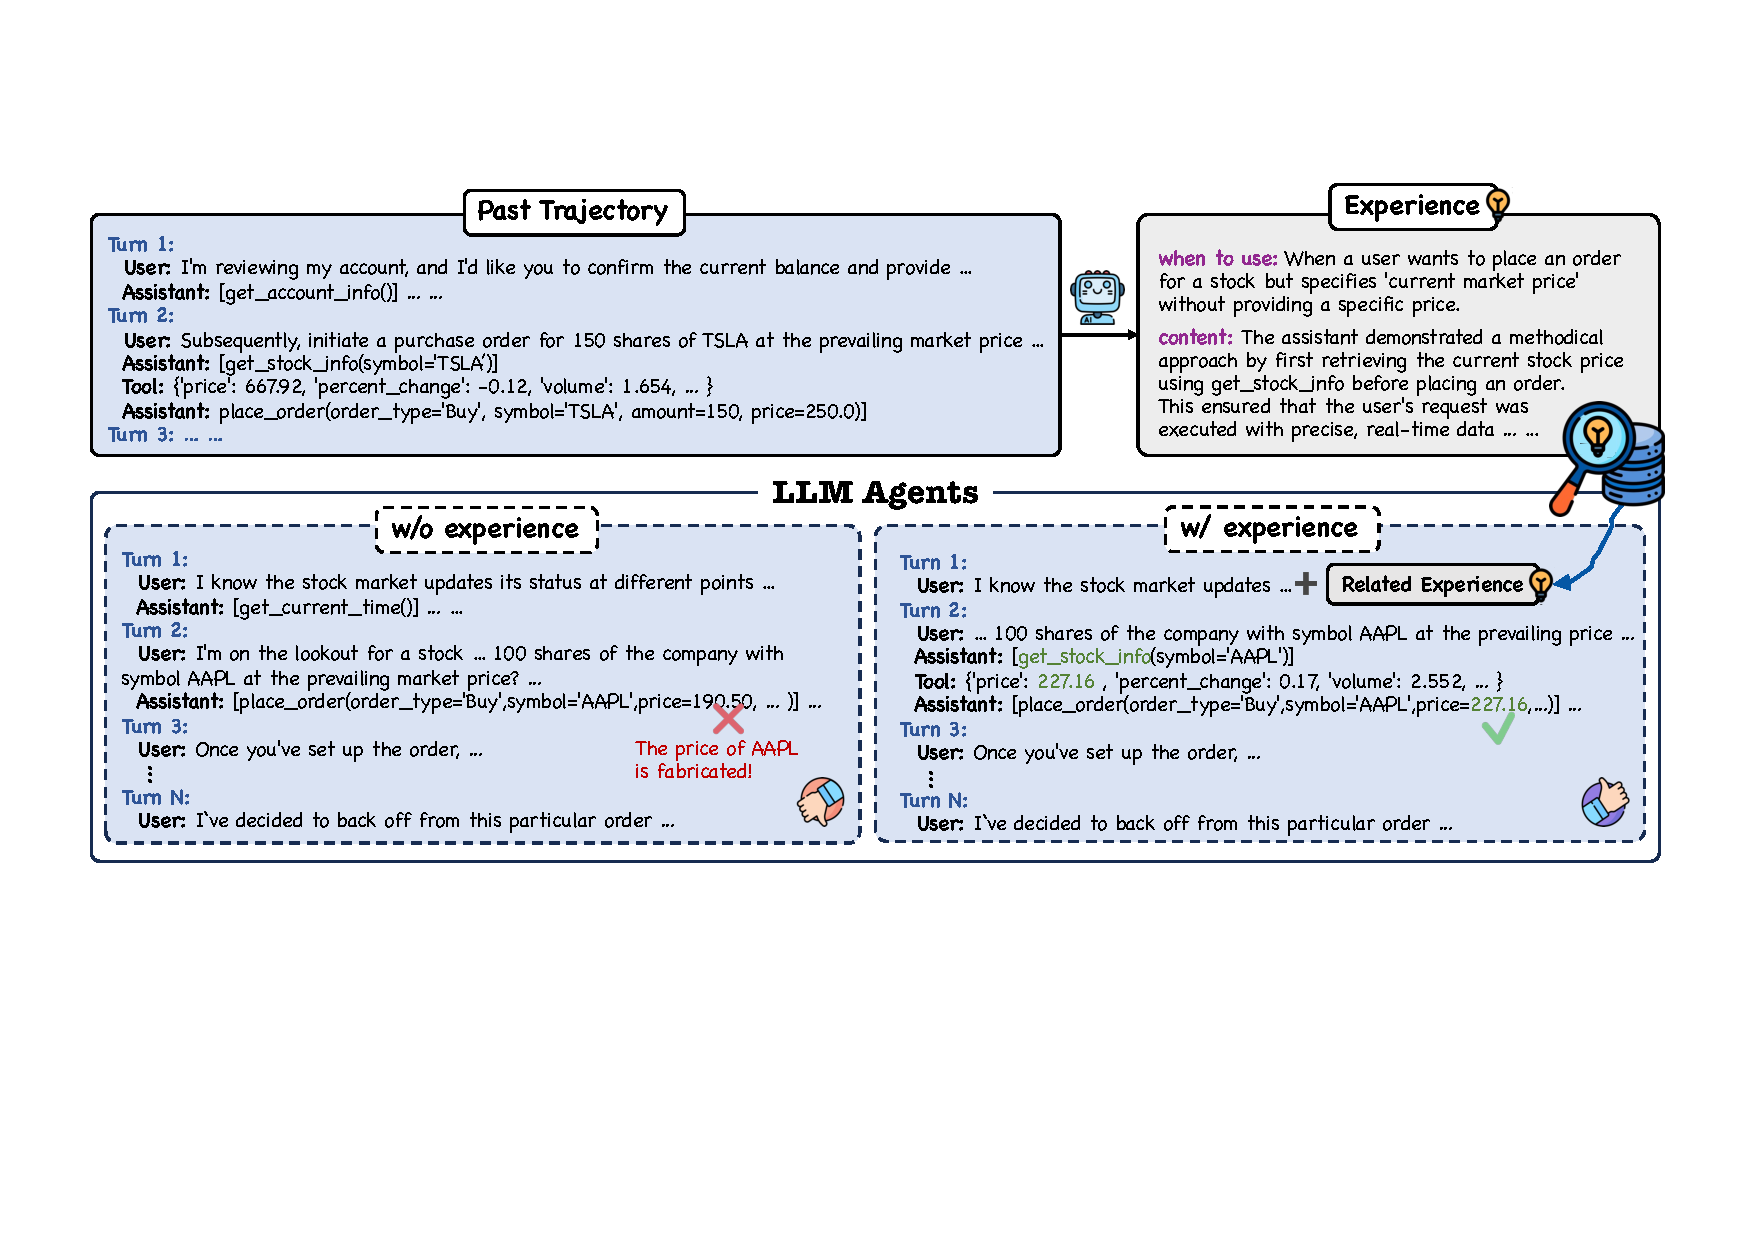
\includegraphics[width=1\linewidth]{figures/example.pdf}
    \caption{Example of how agents complete one stock trading task with and without past experience.}\label{fig:example}
\end{figure*}

In this work, we propose {\ours}, a procedural memory framework that focuses on keypoint-level experience collection for LLM agents. 
Our goal is to maintain a dynamic, high-quality experience pool that enables agents to achieve performance improvement over time. 
Specifically, {\ours} distills key steps from past execution trajectories into structured, reusable experiences, including success pattern recognition, failure analysis and comparative insights. 
When faced with a new task, {\ours} recalls relevant experiences, guiding the agent to avoid blind exploration and allowing it to leverage prior knowledge for enhanced problem-solving capability. 
{\ours} further introduces an experience refinement strategy to maintain the long-term quality of the experience pool that only incorporates new experiences from successful trajectories for reliability and periodically removes ineffective experiences based on their utility. 


Experiments on BFCL-V3 and AppWorld benchmarks show that {\ours} significantly enhances agent performance, with Qwen3-8B improving Avg@4 from 40.33\% to 46.33\% on BFCL-V3 and from 14.97\% to 30.75\% on AppWorld. % on average?
Our ablation studies reveal that fine-grained keypoint-level experiences bring greater performance gains than coarse-grained trajectory-level ones. 
Also, {\ours} significantly enhances experience pool resilience in dynamic environments through our designed robust experience refinement strategy. 
Moreover, lessons from failure trajectories support agent self-reflection, facilitating the exploration on viable solutions.
Overall, we summarize the key contributions as follows: 
\begin{itemize}[leftmargin=12pt,topsep=2pt,itemsep=-2pt]
    \item We present {\ours}, a simple yet effective memory framework that leverages procedural memory (i.e., experience) to continuously enhance agent performance over time.
    \item We validate the advantage of collecting experiences at a fine-grained level over coarse-grained approaches. Our experience refinement mechanism further enables a self‑evolving experience pool that guides long‑term agent behavior.
    \item Experimental results reveal that {\ours} achieves superior agent performance compared to other baselines. Moreover, extensive ablation studies on memory design provide actionable insights for experience-driven agent evolution.
\end{itemize}


